\section{广义积分与含参变量的积分}

\subsection{复习要点}

\subsubsection{学习提示}

本章介绍的广义积分主要分为两大类：
\textbf{无穷积分}和\textbf{瑕积分}.
本讲义将以讲解无穷积分为主，
即如下积分限取无穷大极限时的积分值：
\begin{eq1}
    \int_{a}^{+\infty} f(x) ~\d x = \lim\limits_{A \to +\infty} \int_{a}^{A} f(x) ~\d x
\end{eq1}

而瑕积分原则上都可以通过换元法转换为无穷积分.
设$x \to a^{+}$时$f(x)$无界，即$a$为\textbf{瑕点}.
则瑕积分的定义及变换得到的无穷积分是：
\begin{eq1}
    \int_{a}^{b} f(x) ~\d x =
    \lim\limits_{\epsilon \to 0^{+}} \int_{a+\epsilon}^{b} f(x) ~\d x
    \xlongequal{t = \frac{1}{x-a}} \int_{1/(b-a)}^{+\infty} \frac{f(\frac{1}{t}+a)}{t^2} ~\d t
\end{eq1}

这个换元的合理性需要通过定义来说明（例\ref{ex:ch11-01}），
但是一般情况下，可以不加证明地使用.
当然这并不意味着可以把教材上关于瑕积分的叙述直接撕下来扔掉了，
因为总会出现用不了这种换元法的情况.
不过总体上说，只要掌握了无穷积分，
瑕积分就没有任何有新意的内容了.
接下来说明几项学习的要点：\vspace{0.5em}

(1) ~拿到一个积分首先要分析它属于什么类型，以及要把它拆解为多少个广义积分来处理.
这两个步骤都很容易出错.
关于第一点，积分上限带有“$\infty$”的不一定只是无穷积分.
需要注意积分区间内有没有瑕点，可能既是无穷积分又是瑕积分.
关于第二点，则涉及到对于定义的理解.
举下面两个例子：
\begin{eq1}
    I_1 = \int_{-\infty}^{+\infty} x ~\d x
    ~~~~~~~~~~~
    I_2 = \int_{-1}^{1} \frac{1}{x} ~\d x
\end{eq1}

有同学可能认为这两个积分都收敛，
理由是被积函数是奇函数，
且积分区间都关于$0$对称，
左右抵消结果为$0$.
有这种想法很自然，
可惜这并非我们教材所采用的定义，
所以只能算错误.
正确的分析是，
这两个积分都应该拆成两个广义积分相加：
\begin{eq1}
    I_1 &= \int_{-\infty}^{\infty} x~\d x = \int_{-\infty}^{0} x~\d x + \int_{0}^{\infty} x~\d x  \\
    I_2 &= \int_{-1}^{1} \frac{1}{x} ~\d x = \int_{-1}^{0} \frac{1}{x} ~\d x + \int_{0}^{1} \frac{1}{x} ~\d x
\end{eq1}

无论是$I_1$还是$I_2$，
经拆解后，
在两个子区间上都发散.
所以$I_1$和$I_2$是发散的.

这两个例子说明，在分析广义积分的收敛性时，
必须先对积分区间进行拆分，
使得每个区间内只含有单侧的无穷大或者单侧的瑕点.\vspace{0.5em}

(2) ~本章的定理繁多，需要把每个定理的条件都记清楚.
在学习时关注无穷积分和级数之间的相似之处是记忆的捷径.
具体来说，无穷积分的许多性质和定理可以与数项级数类比，
含参变量无穷积分的许多性质和定理可以与函数项级数类比.
这里，我们首先列出级数和无穷积分的一些基本概念和符号的对应关系，
供大家参考.
表格中左侧和右侧的概念是一一对应的.\vspace{0.5em}

\begin{table}[!ht]
    \centering
    \renewcommand{\arraystretch}{2.25}
    \begin{tabular}{|C{6cm}|C{6cm}|}
    \hline
        \textbf{数项级数}$\sum_{n=1}^{\infty} a_n $ & \textbf{无穷积分}$\int_{a}^{+\infty} f(x) ~\d x $ \\ \hline
        级数通项$a_n$ & 被积函数$f(x)$ \\ \hline
        通项角标$n$ & 被积函数自变量$x$ \\ \hline
        级数部分和$S_N = \sum_{n=1}^{N} a_n$ & “部分积分”$I(A) = \int_{a}^{A} f(x)~\d x$ \\ \hline
        极限过程：$N \to \infty$ & 极限过程：$A \to +\infty$ \\ \hline
        绝对收敛：$\sum_{n=1}^{\infty} |a_n| $收敛 & 绝对收敛：$\int_{a}^{+\infty} |f(x)| ~\d x $收敛 \\ \hline
        \textbf{函数项级数}$\sum_{n=1}^{\infty} f_n(x) $ & \textbf{含参变量无穷积分}$\int_{a}^{+\infty} f(x,y) ~\d x $ \\ \hline
        函数自变量$x$ & 参变量$y$ \\ \hline
    \end{tabular}
\end{table}

(3) ~本章的课本例题十分重要，十分建议大家全都仔细地做一遍.
本章的题目既要求计算能力，也要求严谨性.
而例题既展示了规范的解题方法，也可以作为经典例子积累下来.
考试题与教材例题相似的可能性很高.

\subsubsection{广义积分相关定理简述（注意和级数相关定理类比）}

\setstretch{2.25}
\textbf{1.}~~\textbf{柯西收敛原理}：无穷积分收敛的等价条件是，只要$A$和$A'$都充分大（$>A_0$），必能让
$\left| \int_{A}^{A'} f(x)~\d x \right|$充分小（$<\epsilon$）.\vspace{0.5em}

\textbf{2.}~~\textbf{无穷积分绝对收敛能推出收敛.} 收敛但不绝对收敛称为\textbf{条件收敛}.\vspace{0.5em}

\setstretch{1.75}

\textbf{3.}~~当被积函数$f(x)$非负，则无穷积分收敛当且仅当部分积分$I(A) = \int_{a}^{A} f(x)~\d x$有上界.\vspace{0.5em}

\textbf{4.}~~\textbf{比较判别法：}若两个被积函数都非负，大积分收敛可以推出小积分收敛，小积分发散可以推出大积分发散.\vspace{0.5em}

\textbf{5.}~~\textbf{比较判别法的极限形式：}若两个被积函数都非负，且$x \to +\infty$时二者是同阶无穷小量，则两个积分敛散性相同.\vspace{0.5em}

\textbf{6.}~~\textbf{狄利克雷判别法：}$\int_{a}^{A} f(x)~\d x$有界 + $g(x)$单调趋于$0$ $\Rightarrow$ $\int_{a}^{+\infty} f(x)g(x) ~\d x $收敛. \vspace{0.5em}

\textbf{7.}~~\textbf{阿贝尔判别法：}$\int_{a}^{+\infty} f(x)~\d x$收敛 + $g(x)$单调有界 $\Rightarrow$ $\int_{a}^{+\infty} f(x)g(x) ~\d x $收敛.

\subsubsection{广义积分实用结论}

\textbf{1.}~~$\int_{a}^{+\infty} \frac{1}{x^{p}}~\d x$，$p \in \mathbb{R}$，$a>0$. （教材11.1正文举例，由定义得出）\vspace{0.5em}

~~~~(I)~当$p>1$，无穷积分收敛.

~~~~(II)~当$p \le 1$，无穷积分发散. \vspace{1em}

\textbf{2.}~~$\int_{a}^{+\infty} \frac{1}{x^{p} \ln^q x }~\d x$，$p,q \in \mathbb{R}$，$a>1$. （换元法） \vspace{0.5em}

~~~~(I)~当$p>1$，无穷积分收敛.

~~~~(II)~当$p<1$，无穷积分发散.

~~~~(III)~当$p=1$，无穷积分的敛散性才由对数项决定：

~~~~~~~~(1)~当$q > 1$，无穷积分收敛.

~~~~~~~~(2)~当$q \le 1$，无穷积分发散. \vspace{1em}

\textbf{3.}~~$\int_{a}^{+\infty} \frac{\sin x}{x^p} ~\d x$，
$\int_{a}^{+\infty} \frac{\cos x}{x^p} ~\d x$，
$p \in \mathbb{R}$，$a>0$. （教材11.1例8） \vspace{0.5em}

~~~~(I)~当$p>1$，绝对收敛. （比较判别法）

~~~~(II)~当$0<p \le 1$，条件收敛. （狄利克雷判别法）

~~~~(III)~当$p \le 0$，发散. （转化为级数）\vspace{1em}

\textbf{4.}~~$\int_{0}^{a} \frac{1}{x^{p}}~\d x$，$p \in \mathbb{R}$，$0<a<1$. （教材11.1例10）\vspace{0.5em}

~~~~(I)~当$p < 1$，瑕积分收敛.

~~~~(II)~当$p \ge 1$，瑕积分发散. \vspace{1em}

\textbf{5.}~~$\int_{0}^{a} \frac{1}{x^p \ln^q x}~\d x$，$p \in \mathbb{R}$，$q \in \mathbb{Q}$，$0<a<1$. （比较判别法/换元法） \vspace{0.5em}

~~~~(I)~当$p<1$，无穷积分收敛.

~~~~(II)~当$p>1$，无穷积分发散.

~~~~(III)~当$p=1$，无穷积分的敛散性才由对数项决定：

~~~~~~~~(1)~当$q > 1$，无穷积分收敛.

~~~~~~~~(2)~当$q \le 1$，无穷积分发散. \vspace{1em}

\subsubsection{含参变量正常积分的换序问题}

在正常一元函数定积分的基础上，我们考虑被积函数$f(x)$中除了积分变量$x$以外还含有一个参变量$y$的情况.
此时被积函数可以记为关于$x$和$y$的二元函数$f(x,y)$.
而积分可以看成关于参变量$y$的函数：
\begin{eq1}
    g(y) = \int_{a}^{b} f(x,y) ~\d x
\end{eq1}

对于此类函数的讨论仍然是“老三样”：\textbf{连续性}、\textbf{可积性}和\textbf{可微性}.
在有了这些性质之后，我们特别关心此类函数求极限、定积分和导数的方法.
因此同时也提出了极限/积分/求导与积分号能换序的充分条件.

各项定理有一条共同的前置条件：\textbf{二元函数$f(x,y)$在闭矩形域$\overline{R}:[a,b]\times [c,d]$上连续.} \vspace{1em}

\textbf{1.}~~\textbf{连续性：}参变量积分$g(y)$在$[c,d]$上连续.\vspace{0.5em}
进一步，求极限与积分可换序，即：
\begin{eq1}
    \lim\limits_{y \to y_0} \int_{a}^{b} f(x,y)~\d x
    =\int_{a}^{b} \lim\limits_{y \to y_0}  f(x,y)~\d x
\end{eq1}

（注：书上举出$f(x,y)=\frac{x}{y^2}e^{-x^2/y^2}$的例子来说明，当二元函数连续性不满足，极限和积分号不一定可换序.
可以借助这个例子深入思考其中的原理. 提示：考虑$f(x,y)$当$y \to 0$时收敛到$0$的速度，是否一致收敛？）\vspace{0.5em}

\textbf{2.}~~\textbf{可积性：}参变量积分$g(y)$在$[c,d]$上可积，
且两个积分号可换序，即：
\begin{eq1}
    \int_{c}^{d} \d y \int_{a}^{b} f(x,y)~\d x =
    \int_{a}^{b} \d x \int_{c}^{d} f(x,y)~\d y
\end{eq1}

（注：此事在第七章中亦有记载.）\vspace{0.5em}

\textbf{3.}~~\textbf{可微性：额外要求$f_y (x,y)$也在闭矩形域$\overline{R}$上连续.}
此时参变量积分$g(y)$在$[c,d]$上可微，且求导和积分号可换序，即：
\begin{eq1}
    g'(y) = \frac{\d }{\d y} \int_{a}^{b} f(x,y)~\d x =
     \int_{a}^{b} f_y (x,y)~\d x
\end{eq1}

\subsubsection{含参变量广义积分I：一致收敛}

本节进一步研究含参变量的广义积分：
\begin{eq1}
    g(y) = \int_{a}^{+\infty} f(x,y)~\d x
\end{eq1}

最终的目的还是回答有关$g(y)$连续性、可积性、可微性以及相应的换序问题.
我们十分期待相关的定理与上一节含参变量正常积分完全一致——
实际上确实差不多，只不过广义积分还涉及到收敛性的问题.
教材11.3节开头的分析告诉我们：$g(y)$如果只满足\textbf{点点收敛}，
即便$f(x,y)$对任意$y$连续，$g(y)$也不一定连续.
所以在收敛性这方面，我们需要一个更强的限制条件，即\textbf{一致收敛}.

对于一致收敛的解读在级数章节已经有了，这里不再重复.
我们列举含参变量广义积分一致收敛的相关定理（部分定理简述，帮助记忆）：\vspace{1em}

\textbf{1.}~~\textbf{定义：}若无穷积分$g(y) = \int_{a}^{+\infty} f(x,y) ~\d x$对于区间$Y$中的一切$y$都收敛（点点收敛）.
若对任给$\epsilon >0$，存在一个\textbf{与$y$无关}的实数$N>a$，使当$A>N$时，对一切$y \in Y$都有：
\begin{eq1}
    \left| \int_{A}^{+\infty} f(x,y)~\d x \right| < \epsilon
\end{eq1}

则称含参变量无穷积分$g(y)$在$Y$上一致收敛.\vspace{1em}

\textbf{2.}~~\textbf{柯西收敛准则：}含参变量无穷积分在区间$Y$上一致收敛的充要条件是，对任给$\epsilon > 0$，
存在与$y$无关的实数$N$，使当$A>N$，$A'>N$时，对一切$y \in Y$，都有
\begin{eq1}
    \left| \int_{A}^{A'} f(x,y)~\d x \right| < \epsilon
\end{eq1}

（注：与不含参变量的无穷积分的柯西收敛准则完全相同，只是强调了$N$的选取与$y$无关.）

\vspace{1em}

\textbf{3.}~~\textbf{Weierstrass-M判别法：}假设在积分区间内，被积函数$f(x,y)$能被一个（与$y$无关的）函数$\varphi (x)$控制，即：
\begin{eq1}
    |f(x,y)| \le \varphi (x)
\end{eq1}

且无穷积分$\int_{a}^{+\infty} \varphi (x)~\d x$收敛，
则$\int_{a}^{+\infty} f(x,y)~\d x$一致收敛. \vspace{0.25em}

（注：即函数项级数一致收敛的强级数判别法. 该判别法只能判断绝对一致收敛.）\vspace{1em}

\textbf{4.}~~\textbf{狄利克雷判别法：}部分积分$\int_{a}^{A} f(x,y) ~\d x$一致有界
+ $g(x,y)$对$x$单调一致趋于$0$

$\Rightarrow$ $\int_{a}^{+\infty} f(x,y)g(x,y)~\d x$一致收敛.

（注：在原版的狄利克雷判别法的基础上，加上一致性的限制即可.）\vspace{1em}

\textbf{5.}~~\textbf{阿贝尔判别法：}$\int_{a}^{+\infty} f(x,y)~\d x$一致收敛 + $g(x,y)$单调一致有界

$\Rightarrow$ $\int_{a}^{+\infty} f(x,y)g(x,y)~\d x$一致收敛.\vspace{0.25em}

（注：在原版的阿贝尔判别法的基础上，加上一致性的限制即可.）\vspace{1em}

\subsubsection{含参变量广义积分II：换序问题}

如果已知函数$f(x,y)$在区域$[a,+\infty) \times [c,d]$上连续，
且积分$g(y) = \int_{a}^{+\infty} f(x,y)~\d x$在$[c,d]$上一致收敛
（在实际的计算题中，常常要先用前述的判别法证明一致收敛性.），
我们首先可以得到连续性和可积性:\vspace{0.5em}

\textbf{1.}~~\textbf{连续性：}$g(y)$在$[c,d]$上连续，且极限和无穷积分可换序，即：
\begin{eq1}
    \lim\limits_{y \to y_0} \int_{a}^{+\infty} f(x,y)~\d x
    =  \int_{a}^{+\infty} \lim\limits_{y \to y_0} f(x,y)~\d x
\end{eq1}

\textbf{2.}~~\textbf{可积性：}$g(y)$在$[c,d]$上可积，且正常积分和无穷积分可换序，即：
\begin{eq1}
    \int_{c}^{d} \d y \int_{a}^{+\infty} f(x,y)~\d x =
    \int_{a}^{+\infty} \d x \int_{c}^{d} f(x,y)~\d y
\end{eq1}

（注：此处谈论的是正常积分与无穷积分换序. 无穷积分与无穷积分的换序有另一个定理.） \vspace{1em}

在此基础上，若再有$f_y (x,y)$在区域$[a,+\infty) \times [c,d]$上连续，
且积分$\int_{a}^{+\infty} f_y (x,y)~\d x $在$[c,d]$上一致收敛，还能得到可微性：

\textbf{3.}~~\textbf{可微性：}$g(y)$在$[c,d]$上可导，且求导和无穷积分可换序，即：
\begin{eq1}
    g'(y) = \frac{\d}{\d y} \int_{a}^{+\infty} f(x,y)~\d y
    = \int_{a}^{+\infty} f_y (x,y)~\d y
\end{eq1}

\textbf{4.}~~\textbf{无穷积分换序：}设$f(x,y)$在区域$[a,+\infty) \times [c,+\infty)$上连续，又设两个含参变量无穷积分：
\begin{eq1}
    \int_{a}^{+\infty} f(x,y)~\d x ~~~~\text{与}~~~~\int_{c}^{+\infty} f(x,y)~\d y
\end{eq1}
分别关于$y$和$x$在任意又穷闭区间$[c,d]$及$[a,b]$上一致收敛，
并且两积分：
\begin{eq1}
    \int_{a}^{+\infty} \d x \int_{c}^{+\infty} |f(x,y)| ~\d y
    ~~~~\text{与}~~~~
    \int_{c}^{+\infty} \d y \int_{a}^{+\infty} |f(x,y)| ~\d x
\end{eq1}
中至少有一个存在，则两积分：
\begin{eq1}
    \int_{a}^{+\infty} \d x \int_{c}^{+\infty} f(x,y) ~\d y
    ~~~~\text{与}~~~~
    \int_{c}^{+\infty} \d y \int_{a}^{+\infty} f(x,y) ~\d x
\end{eq1}
都存在且相等，即可以交换积分次序.

\subsubsection{$\Gamma$函数和B函数}

$\Gamma$函数的定义如下：
\begin{eq1}
    \Gamma (\alpha) = \int_{0}^{+\infty} x^{\alpha - 1} e^{-x} ~\d x ,~~\alpha > 0
\end{eq1}

其重要性质和公式整理如下：

\textbf{1.}~~$\Gamma (\alpha)$在$(0,+\infty)$上连续.

\textbf{2.}~~$\Gamma (1) = 1$，$\Gamma \left(\frac{1}{2}\right) = \sqrt{\pi}$.

\textbf{3.}~~递推公式：$\Gamma(\alpha + 1) = \alpha \Gamma (\alpha)$.

\textbf{4.}~~与阶乘的关系：当$n \in \mathbb{N}$，$\Gamma (n+1) = n!$.~~（注意不是$\Gamma (n) = n!$）

\textbf{*5.}~~余元公式：$\Gamma (z) \Gamma (1-z) = \frac{\pi}{\sin \pi z}$.~~（注意不要写成$\frac{\pi}{\sin \pi^z}$（狗头））

\textbf{*6.}~~Stirling公式：当$z \to \infty$，$\Gamma (z) \sim z^{z-1/2} e^{-z} \sqrt{2\pi}$.
或者：当$n \to \infty$，$n! \sim \sqrt{2\pi n} \left( \frac{n}{e} \right)^{n}$.\vspace{1em}

B函数的定义如下：
\begin{eq1}
    \text{B}(p,q) = \int_{0}^1 x^{p-1} (1-x)^{q-1} ~\d x ,~~p >0,~~ q>0
\end{eq1}

还有一个三角函数的等价定义：
\begin{eq1}
    \text{B}(p,q) = 2 \int_{0}^{\pi / 2} \cos^{2p-1} \theta \sin^{2q-1} \theta ~\d \theta , ~~p >0,~~ q>0
\end{eq1}

其重要性质和公式整理如下：

\textbf{1.}~~B函数在$(0,+\infty) \times (0,+\infty)$上连续.

\textbf{2.}~~对称性：$\text{B}(p,q) = \text{B}(q,p)$.\vspace{0.2em}

\textbf{3.}~~B$(p,q) = \frac{\Gamma (p) \Gamma (q)}{\Gamma (p+q)}$.

\subsection{解题方法}

\subsubsection{广义积分收敛性判断}

广义积分收敛性的判断，常规题型分为两类：
(1)~如果是非负函数（判断绝对收敛性），
以比较判别法为主，尤其是要和$p$级数比较.
当被积函数较复杂时，可以用泰勒展开，估计被积函数的无穷小阶数.
(2)~如果是一般的正负交替的函数（判断条件收敛性），尤其是带三角函数的形式，
应该设法利用狄利克雷判别法或者达朗贝尔判别法（在课内几乎没有别的方法可用）.\par

注意事项：

(1)~对于抽象的被积函数（没有给$f(x)$的具体表达式），往往要回归广义积分的定义.

(2)~首先要判断清楚广义积分的类型，特别要小心一个积分可能既是无穷积分，又是瑕积分.
此时收敛性需要分开讨论.

(3)~注意判断被积函数是否非负（或非正），不同情况适用不同的判别法.

\begin{example}
\label{ex:ch11-01}
设$f(x)$在$(0,a]$上连续的正值函数，且$x \to 0^{+}$时$f(x)$无界.

(1)~~证明：可以对瑕积分$\int_{0}^{a} f(x) ~\d x$做变量替换$t = \frac{1}{x}$，将其转化为无穷积分.
且瑕积分和无穷积分的收敛性一致.

(2)~~又设$f(x)$在$(0,a]$上严格单调递减.
证明：瑕积分$\int_{0}^{a} f(x) ~\d x$与反函数的无穷积分$\int_{f(a)}^{+\infty} f^{-1}(y) ~\d y$的敛散性一致.
\end{example}

\begin{analysis}
本题的结论提供了两种无穷积分与瑕积分互化的思路.
    两个结论都很易于理解，但是并不显然，需要从定义出发加以论证.

    第一小问，是证明积分的换元法可以用在无穷积分和瑕积分上.
    这个结论之所以需要证明，是因为之前所学的积分换元法是针对于黎曼定积分的，
    而本章所学的广义积分是对黎曼积分的上下限取极限得到的，其本身并不是黎曼积分.
    在证明时也需体现这个极限过程.

    第二小问，是证明如果把整个坐标平面以$y=x$为轴镜像翻转，那么瑕积分可以看成其反函数的无穷积分.
    这在几何意义上是说得通的，因为无穷积分和瑕积分都可以看成函数曲线与$x$轴围成的面积.
    镜像翻转的操作无非是把图像从“无限向上延伸”（瑕积分）变成了“无限向右延伸”（无穷积分）.
    但是问题在于，
    瑕积分的定义并不是由无穷积分“镜像翻转”得到的.
    它们的区别就像是：对于同一块区域，可以沿$x$轴方向无限分割再取极限，也可以沿$y$轴方向无限分割再取极限.
    对于无界区域而言，这两种计算面积的方法一定得到相同的结果吗？这一点需要从定义出发证明.
\end{analysis}

\begin{proof}
(1)~~
    \begin{eq1}
        \int_{0}^{a} f(x)~\d x
        &= \lim\limits_{\delta \to 0^{+}} \int_{\delta}^{a} f(x) ~\d x \\
        &= \lim\limits_{\delta \to 0^{+}} \int_{1/a}^{1/\delta} \frac{f(1/t)}{t^2} ~\d t \\
        &= \lim\limits_{A \to +\infty} \int_{1/a}^{A} \frac{f(1/t)}{t^2} ~\d t
        &= \int_{1/a}^{+\infty} \frac{f(1/t)}{t^2} ~\d t
    \end{eq1}

    (2)~~令$y = f(x)$，即$x = f^{-1}(y)$，则有：
    \begin{align*}
        \int_{f(a)}^{+\infty} f^{-1}(y) ~\d y
        &= \lim\limits_{A \to +\infty} \int_{f(a)}^{A} f^{-1}(y) ~\d y \\
        &= \lim\limits_{A \to +\infty} \int_{a}^{f^{-1}(A)} x ~\d f(x) \\
        &= \lim\limits_{A \to +\infty}  \left( xf(x) \bigg|_{a}^{f^{-1}(A)} + \int_{f^{-1}(A)}^{a} f(x) ~\d x\right) \\
        &= \lim\limits_{\delta \to +0} \left( xf(x) \bigg|_{a}^{\delta} + \int_{\delta}^{a} f(x) ~\d x\right) \\
        &= \lim\limits_{\delta \to +0} \left( \delta f(\delta) - af(a) + \int_{\delta}^{a} f(x) ~\d x\right)~~~~~~(*)
    \end{align*}

    $(*)$式的第三项是瑕积分$\int_{0}^{a} f(x) ~\d x$的定义，
    但不能直接得到无穷积分与瑕积分等价，因为$\delta f(\delta)$的收敛性是未知的.
    接下来我们对此进行讨论：

    i)~~若$\lim\limits_{\delta \to 0^{+}} \delta f(\delta)$存在. 则：
    \begin{eq1}
        \int_{f(a)}^{+\infty} f^{-1}(y) ~\d y
        &= - a f(a) + \lim\limits_{\delta \to 0^{+}} \delta f(\delta)   + \lim\limits_{\delta \to +0} \int_{\delta}^{a} f(x) ~\d x \\
        &=- a f(a) + \lim\limits_{\delta \to 0^{+}} \delta f(\delta)   + \int_{0}^{a} f(x)~\d x
    \end{eq1}

    故$\int_{f(a)}^{+\infty} f^{-1}(y) ~\d y$与$\int_{0}^{a} f(x)~\d x $收敛性一致.

    ii)~~若$\lim\limits_{\delta \to 0^{+}} \delta f(\delta) = +\infty$，
    即$\lim\limits_{\delta \to 0^{+}} \frac{f(\delta)}{1/ \delta} = +\infty$.
    已知瑕积分$\int_{0}^{a} \frac{1}{x} ~\d x$发散.
    由比较判别法可知瑕积分$\int_{0}^{a} f(x)~\d x$也发散$(\to +\infty)$.
    进而由$(*)$式可知无穷积分也发散$(\to +\infty)$.

    综合i)，ii)可知，瑕积分$\int_{0}^{a} f(x) ~\d x$与无穷积分$\int_{f(a)}^{+\infty} f^{-1}(y) ~\d y$同时收敛或同时发散.
\end{proof}

\begin{example}
\label{ex:ch11-02}
设无穷积分$\int_{1}^{+\infty} \left( e^{-\cos \frac{1}{x}} - e^{-1} \right) x^k ~\d x$收敛. 求$k$的范围.
\end{example}

\begin{analysis}
被积函数是非负函数.
    根据比较判别法，只需要估计出被积函数无穷小量阶数.
    可以利用等价无穷小代换/中值定理/泰勒展开等求极限的方法.
\end{analysis}

\begin{solution}
当$x \to +\infty$时，有如下的等价无穷小关系：
    \begin{eq1}
        e^{-\cos \frac{1}{x}} - e^{-1}
        &= e^{-1} \left( e^{1 - \cos \frac{1}{x}} - 1 \right)\\
        &\sim e^{-1} \left( 1 - \cos \frac{1}{x} \right) \\
        &\sim \frac{1}{2ex^2}
    \end{eq1}

    替换被积函数，可知原积分的敛散性与$\int_{1}^{+\infty} \frac{1}{2ex^{2-k}} ~\d x$一致.
    故$k < 1$.
\end{solution}

\begin{example}[2023]
\label{ex:ch11-03}
讨论无穷积分$\int_{1}^{+\infty} \frac{\sin x}{\sqrt{x}} \arctan x$的敛散性.
\end{example}

\begin{analysis}
被积函数不是非负函数，考虑用狄利克雷或阿贝尔判别法.
    这里$\sin x$是典型的变上限积分有界的函数.
    因此根据狄利克雷判别法，只需证明其余部分单调趋于$0$.
\end{analysis}

\begin{solution}
$\sin x$的变上限积分有界：
    \begin{eq1}
        \left|\int_{1}^{A} \sin x ~\d x \right|
        = \left| -\cos A + \cos 1 \right| \le 2
    \end{eq1}

对其余部分$g(x) = \frac{\arctan x}{\sqrt{x}}$求导：
\begin{eq1}
    g'(x)
    = \frac{1}{\sqrt{x}(1+x^2)} - \frac{\arctan x}{2x^{3/2}} = \frac{1}{x^{3/2}} \left( \frac{x}{1+x^2} - \frac{\arctan x}{2} \right)
\end{eq1}

可知$g'(x)$在定义域内单调递减. 由$g'(2)<0$，可知$x > 2$时$g'(x) < 0$，
即$g(x)$单调递减.

计算$g(x)$的极限：
\begin{eq1}
    \lim\limits_{x \to +\infty} g(x)
    = \lim\limits_{x \to +\infty}  \frac{\arctan x}{\sqrt{x}}
    = 0
\end{eq1}

由狄利克雷判别法，该无穷积分收敛.
\end{solution}

\begin{example}
\label{ex:ch11-04}
若积分$\int_{0}^{1} \frac{\ln x}{x^p (1-x)^{1-p}} ~\d x$收敛.
        求$p$的取值范围.
\end{example}

\begin{analysis}
此题要注意$x=0^{+}$和$x=1^{-}$都可能是瑕点.
    需要保证这两处瑕积分都收敛.
\end{analysis}

\begin{solution}
被积函数在$(0,1)$上非正.
    现分别考虑$x=0$和$x=1$处的收敛性.

    i)~~考虑积分$\int_{0}^{1/2} \frac{\ln x}{x^p (1-x)^{1-p}} ~\d x$.
    因为当$x \to 0^{+}$时，$(1-x)^{1-p} \to 1$，所以该积分的敛散性与
    $\int_{0}^{1/2} \frac{\ln x}{x^{p}}~\d x$一致.
    由讲义11.1.3的结论5，该积分收敛当且仅当$p < 1$.
    证明如下：

    当$p \ge 1$时，$\frac{\ln x}{x^{p}} \le \frac{\ln \frac{1}{2}}{x}$.
    $\int_{0}^{1/2} \frac{\ln \frac{1}{2}}{x} ~\d x$发散.
    由比较判别法可知，$\int_{0}^{1/2} \frac{\ln x}{x^p} ~\d x$发散.

    当$p < 1$时，记$\epsilon = \frac{1-p}{2} > 0$，则$p + \epsilon < 1$，
    瑕积分$\int_{0}^{1/2} \frac{1}{x^{p + \epsilon}} ~\d x$收敛.
    另外：
    \begin{eq1}
        \lim\limits_{x \to 0^{+}} \frac{\ln x / x^{p}}{1/x^{p + \epsilon}}
        = \lim\limits_{x \to 0^{+}} x^{\epsilon} \ln x = 0
    \end{eq1}

    由比较判别法可知，$\int_{0}^{1/2} \frac{\ln x}{x^p} ~\d x$收敛.

    ii)~~考虑积分$\int_{1/2}^{1} \frac{\ln x}{x^p (1-x)^{1-p}}~\d x$.
    因为当$x \to 1^{-}$时，$x^{p} \to 1$，$\ln x \sim \ln (1 + x -1) \sim x - 1$，
    所以该积分的敛散性与$\int_{1/2}^{1} \frac{-1}{(1-x)^{-p}} ~\d x$一致.
    因此$p > -1$.

    综合i)，ii)可知，$-1 < p < 1$.
\end{solution}

\begin{example}
\label{ex:ch11-05}
若$\int_{0}^{2} \frac{1}{|\ln x|^{a}} ~\d x$收敛.
        求$a$的范围.
\end{example}

\begin{analysis}
此题要注意$x=0^{+}$，$x=1^{-}$和$x = 1^{+}$都可能是瑕点.
\end{analysis}

\begin{solution}
将整个积分拆分为：
    \begin{eq1}
        \int_{0}^{2} \frac{1}{|\ln x|^{a}}~\d x
        = \int_{0}^{1/2} \frac{1}{|\ln x|^a}~\d x
        + \int_{1/2}^{1} \frac{1}{|\ln x|^a}~\d x
        + \int_{1}^{2} \frac{1}{|\ln x|^a} ~\d x
    \end{eq1}
    现分别讨论右侧三个瑕积分的收敛性：

    i)~~由讲义11.1.3的结论5，积分$\int_{0}^{1/2} \frac{1}{|\ln x|^a}~\d x$收敛对$a \in \mathbb{R}$成立.

    ii)~~当$x \to 1^{-}$时，$|\ln x| \sim |\ln (1 + x -1)| \sim 1-x$.
    故积分$\int_{1/2}^{1} \frac{1}{|\ln x|^a} ~\d x$的敛散性与
    $\int_{1/2}^{1} \frac{1}{(1-x)^a} ~\d x$一致.
    故$a < 1$.

    iii)~~当$x \to 1^{+}$时，$|\ln x| \sim |\ln (1 + x -1)| \sim x-1$.
    故积分$\int_{1}^{2} \frac{1}{|\ln x|^a} ~\d x$的敛散性与
    $\int_{1}^{2} \frac{1}{(x-1)^a} ~\d x$一致.
    故$a < 1$.

    综合i)，ii)，iii)可知，$a<1$.
\end{solution}

\begin{example}[2021]
\label{ex:ch11-06}
定义函数 \(\theta : [0, +\infty) \to [0, +\infty)\) 为
       \begin{eq1}
            \theta(x) = \int_0^x \sqrt{(t+1)(t+2)(t+3)}  ~\d t
       \end{eq1}
    证明无穷积分
    $\int_0^{+\infty} \cos\left(\theta(x)\right)  ~\d x$收敛.
\end{example}

\begin{analysis}
如果熟悉教材知识点，此题的思路容易想到.
    余弦函数中复合了另一个函数$\theta (x)$，我们是没办法处理的.
    但是对于没有复合的$\cos x$，我们可以利用其变上限积分有界，进而通过狄利克雷判别法证明无穷积分收敛.
    因此，令$s = \theta (x)$，从而把余弦函数“解放出来”，是势在必行的一步.
\end{analysis}

\begin{proof}
令$s = \theta (x)$，则有：
    \begin{eq}
        \d s  = \d \theta (x)
        = \theta'(x) ~\d x
    \end{eq}

    另外：
    \begin{eq}
        \theta '(x) = \sqrt{(x+1)(x+2)(x+3)}
    \end{eq}

    故：
    \begin{eq1}
        \int_{0}^{+\infty} \cos (\theta (x)) ~\d x
        = \int_{x=0}^{x=+\infty} \frac{\cos s ~\d s}{\sqrt{(x+1)(x+2)(x+3)}}
    \end{eq1}

    \setstretch{2.25}

    其中，$\int_{x=0}^{x=A} \cos s ~\d s$有界，
    而$\frac{1}{\sqrt{(x+1)(x+2)(x+3)}}$单调递减趋于$0$.
    根据狄利克雷判别法，
    该无穷积分收敛.
\end{proof}

\setstretch{1.75}

\subsubsection{广义积分的计算}

根据往年的经验，广义积分的计算题是必考的，
而且必考$\Gamma$函数和B函数（不要试图用莱布尼茨公式）.

\begin{example}[2022]
\label{ex:ch11-07}
求无穷积分 \( \int_{0}^{+\infty} \sqrt{x^3 e^{-x}} ~\d x \) 的值，
        和瑕积分 \( \int_{0}^{1} \sqrt{\frac{x^3}{1-x}} ~\d x \) 的值.
\end{example}

\begin{solution}
(1)
    \[ \int_{0}^{+\infty} \sqrt{x^3 e^{-x}} ~\d x = \Gamma\left(\frac{5}{2}\right) = \frac{3}{2} \cdot \frac{1}{2} \Gamma\left(\frac{1}{2}\right) = \frac{3}{4} \sqrt{\pi} \]

    (2)
    \[ \int_{0}^{1} \sqrt{\frac{x^3}{1-x}} ~\d x = \int_{0}^{1} x^{\frac{3}{2}} (1-x)^{-\frac{1}{2}} ~\d x = \text{B} \left(\frac{5}{2}, \frac{1}{2}\right) = \frac{\Gamma\left(\frac{5}{2}\right) \Gamma\left(\frac{1}{2}\right)}{\Gamma(1)} = \frac{\frac{3}{4} \sqrt{\pi} \cdot \sqrt{\pi}}{1} = \frac{3}{4} \pi \]
\end{solution}

\begin{example}[2021]
\label{ex:ch11-08}
(1)求出无穷积分 $\int_{0}^{+\infty} \sqrt{x} e^{-x}  ~\d x $ 的值；

(2)求出瑕积分 $\int_{0}^{1} \frac{1}{\sqrt{x(1-x)}}  ~\d x $ 的值.
\end{example}

\begin{solution}
(1)
    \[ \int_{0}^{+\infty} \sqrt{x} e^{-x}  \d x = \int_{0}^{+\infty} x^{\frac{3}{2}-1} e^{-x}  \d x = \Gamma\left(\frac{3}{2}\right) = \frac{1}{2} \Gamma\left(\frac{1}{2}\right) = \frac{1}{2} \sqrt{\pi} \]

    (2)
    \[ \int_{0}^{1} \frac{1}{\sqrt{x(1-x)}}  \d x = \int_{0}^{1} x^{\frac{1}{2}-1}(1-x)^{\frac{1}{2}-1}  \d x = \text{B} \left(\frac{1}{2}, \frac{1}{2}\right)
    = \frac{\Gamma\left(\frac{1}{2}\right) \Gamma\left(\frac{1}{2}\right)}{\Gamma(1)} = \pi \]
\end{solution}

\begin{example}[2024]
\label{ex:ch11-09}
求积分的值： \[ \int_{0}^{1} \sqrt{\frac{x^5}{1-x}}  ~\d x \] .
\end{example}

\begin{solution}
\begin{eq1}
        \int_{0}^{1} \sqrt{\frac{x^5}{1-x}} ~\d x &= \int_{0}^{1} x^{\frac{5}{2}}(1-x)^{-\frac{1}{2}}  ~\d x = \text{B}\left(\frac{7}{2}, \frac{1}{2}\right) = \frac{\Gamma\left(\frac{7}{2}\right) \Gamma\left(\frac{1}{2}\right)}{\Gamma(4)} \\
        &= \frac{\frac{5}{2} \cdot \frac{3}{2} \cdot \frac{1}{2} \cdot \Gamma\left(\frac{1}{2}\right) \cdot \Gamma \left(\frac{1}{2}\right)}{3!} = \frac{\frac{15}{8} \sqrt{\pi} \cdot \sqrt{\pi}}{6}  = \frac{5}{16} \pi
    \end{eq1}
\end{solution}

\subsubsection{广义积分综合题——级数相关}

\begin{example}[教材11.1例8]
\label{ex:ch11-10}
证明：当$0 < p \le 1$时，积分$\int_{1}^{+\infty} \frac{\sin x}{x^p}~\d x$条件收敛.

\setstretch{2}
\end{example}

\begin{proof}
先证明$\int_{1}^{+\infty} \frac{\sin x}{x} ~\d x$收敛.
    变上限积分$\int_{1}^{+\infty} \sin x ~\d x$有界.
    又因为$p>0$，所以函数$\frac{1}{x^p}$单调递减趋于$0$（当$x \to +\infty$）.
    由狄利克雷判别法即知当$0 < p \le 1$时，
    $\int_{1}^{+\infty} \frac{\sin x}{x^p}~\d x$收敛.

    其次证明$\int_{1}^{+\infty} \left| \frac{\sin x}{x^p} \right| ~\d x$发散.
    为此只须证明当$A \to +\infty$时，$\int_{1}^{A} \left| \frac{\sin x}{x^p} \right| ~\d x $无界.
    不妨设$A > 2\pi$.
    取$\left[ \frac{A}{\pi} \right] = n_0$，
    则有$A \ge n_0 \pi$及$n_0 \ge 2$.
    注意$\left| \frac{\sin x}{x^p} \right|$非负，便有：

    \begin{eq1}
        \int_{1}^{A} \left| \frac{\sin x}{x^p} \right| ~\d x
        &\ge \int_{\pi}^{n_0 \pi} \frac{|\sin x|}{x^p} ~\d x
        = \sum_{n=2}^{n_0} \int_{(n-1)\pi}^{n\pi} \frac{|\sin x|}{x^p} ~\d x \\
        &\ge \sum_{n=2}^{n_0} \frac{1}{(n\pi)^p} \int_{(n-1)\pi}^{n\pi} |\sin x|~\d x \\
        &= \sum_{n=2}^{n_0} \frac{1}{(n\pi)^p} \int_{0}^{\pi} \sin x ~\d x = \frac{2}{\pi^p} \sum_{n=2}^{n_0} \frac{1}{n^p}
    \end{eq1}

    由于$0 < p \le 1$，级数$\sum_{n=2}^{+\infty} \frac{1}{x^p}$发散.
    故$\sum_{n=2}^{n_0} \frac{1}{n^p}$可以大于任意给定的正数，只要$n_0$充分大.
    由此推出$\int_{1}^{A} \frac{|\sin x|}{x^p}~\d x$可大于任意给定的正数，
    只要$A$充分大.
    这即意味着$\int_{1}^{A} \left| \frac{\sin x}{x^p} \right| ~\d x$无界，
    即$\int_{1}^{+\infty} \left| \frac{\sin x}{x^p} \right| ~\d x$发散.

    综合上述，当$0 < p \le 1$时，$\int_{1}^{+\infty} \frac{\sin x}{x^p} ~\d x$条件收敛.
\end{proof}

\setstretch{1.75}

从这道教材例题可以看出，无穷积分和级数有着紧密的关联.
我们把$x$轴分割成了无穷多个
$[(n-1)\pi , n\pi]$区间.
这样，无穷积分就可以看成无穷多个有限区间上的积分的累加，也就是一种级数：
\begin{eq1}
    \int_{\pi}^{+\infty} \frac{|\sin x|}{x^p} ~\d x = \sum_{n=2}^{+\infty} \left(\int_{(n-1)\pi}^{n \pi} \frac{|\sin x|}{x^p} ~\d x \right)
\end{eq1}

注意上面的等号对于非负（非正）的被积函数是成立的.
若已经证明了无穷积分收敛，不论被积函数的符号，等号也成立.
除了这两种情况以外，不能武断地认为等号成立.
不过，这种级数与无穷积分转化的思想是普遍适用的.
再回顾上一道例题的解法：
虽然已经将无穷积分转化成了右侧的级数，
但是$\frac{|\sin x|}{x^p}$在有限区间上的积分仍然无法直接计算.
为了证明级数发散，
此时对级数的通项进行放缩，
放缩之后，每个有限区间上的积分都可以计算，
从而可以判断出级数的敛散性.

这种放缩方法，相比于直接对整个被积函数放缩，往往要精细得多.
事实上，正项级数无穷积分判别法的证明也利用了这个思想（图1），
而且，用的还是最简单的常函数放缩.
放缩前后的无穷积分/级数收敛的速度没有数量级的差异，
敛散性是一致的.

在实际做题过程中，
如何分割$x$轴也是有讲究的.
最常要用到这种方法的是被积函数含有三角函数等周期函数的情况.
那么，对$x$轴的分割应该配合它的周期.
如上例中被积函数有$|\sin x|$，
那就以$\pi$为一个区间长度进行分割.
如果被积函数是正负交替的，
那么可以取被积函数的零点作为分割点，
使得分割后的级数是交错级数.

\begin{figure}[H]
    \centering
    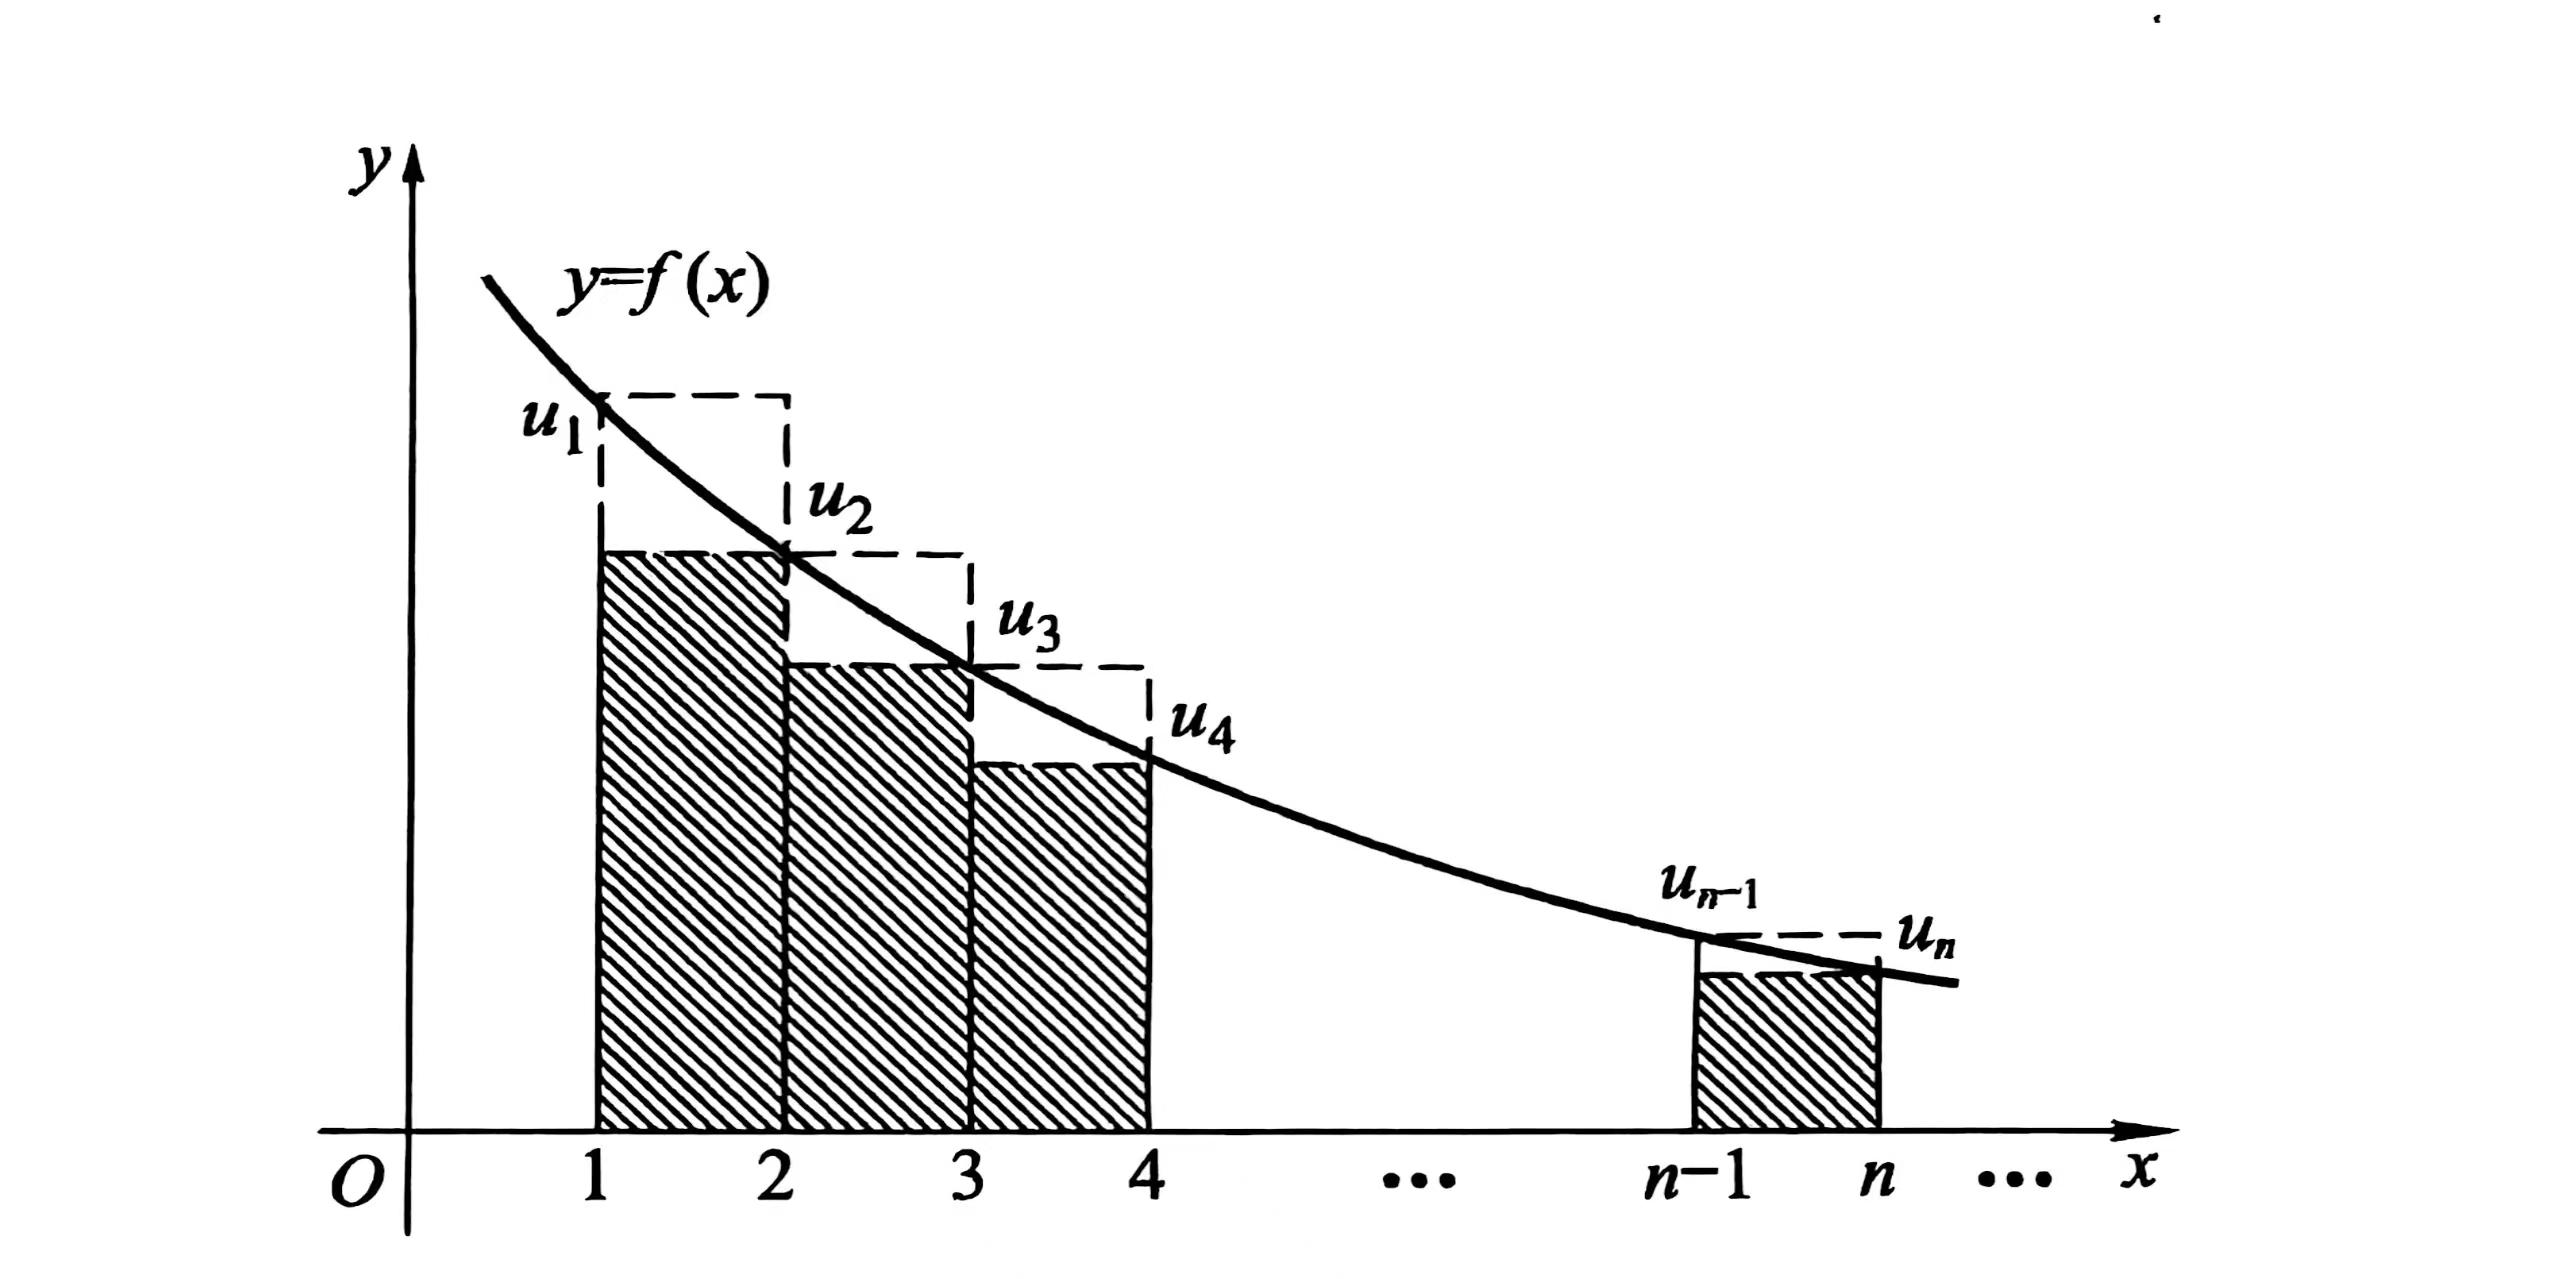
\includegraphics[width=0.8\textwidth]{fig11_1.jpg}
    \caption{无穷积分可以精细地向下（阴影部分面积）和向上（虚线部分面积+阴影部分面积）放缩成级数}
\end{figure}

\begin{example}
\label{ex:ch11-11}
设$\alpha, \beta > 0$.
        若无穷积分$\int_{0}^{+\infty} \frac{x^\alpha ~\d x}{1 + x^{\beta} \sin^2 x}$，
        求$\alpha, \beta$所满足的关系.
\end{example}

\begin{solution}
设$n \in \mathbb{N}$.
    当$x \in [n\pi, (n+1)\pi]$时，被积函数$f(x) = \frac{x^\alpha }{1 + x^{\beta} \sin^2 x}$可放缩如下：
    \begin{eq1}
        \frac{(n\pi)^{\alpha}}{1 + (n+1)^{\beta} \pi^{\beta} \sin^2 x}
        \le f(x)
        \le
        \frac{(n+1)^{\alpha}\pi^{\alpha}}{1 + n^{\beta} \pi^{\beta} \sin^2 x}
    \end{eq1}

    故：
    \begin{eq1}
        \int_{n\pi}^{(n+1)\pi} \frac{(n\pi)^{\alpha}~\d x}{1 + (n+1)^{\beta} \pi^{\beta} \sin^2 x}
        \le
        \int_{n\pi}^{(n+1)\pi} f(x)~\d x
        \le
        \int_{n\pi}^{(n+1)\pi} \frac{(n+1)^{\alpha}\pi^{\alpha} ~\d x}{1 + n^{\beta} \pi^{\beta} \sin^2 x}
    \end{eq1}

    计算出左侧和右侧的积分（过程省略）：
    \begin{eq1}
        \frac{n^{\alpha} \pi^{\alpha + 1}}{\sqrt{1 + (n+1)^{\beta} \pi^{\beta}}}
        \le
        \int_{n\pi}^{(n+1)\pi} f(x)~\d x
        \le
        \frac{(n+1)^{\alpha} \pi^{\alpha + 1}}{\sqrt{1 + n^{\beta} \pi^{\beta}}}
    \end{eq1}

    对上述不等式从$n=0$到$n=\infty$求和：
    \begin{eq1}
        \sum_{n=0}^{+\infty} \frac{n^{\alpha} \pi^{\alpha + 1}}{\sqrt{1 + (n+1)^{\beta} \pi^{\beta}}}
        \le
        \int_{0}^{+\infty} f(x)~\d x
        \le
        \sum_{n=0}^{+\infty} \frac{(n+1)^{\alpha} \pi^{\alpha + 1}}{\sqrt{1 + n^{\beta} \pi^{\beta}}}
    \end{eq1}

    左侧级数和右侧级数都是正项级数，
    且级数通项都与$n^{\alpha - \beta / 2}$同阶（当$n \to \infty$）.
    由$p$级数结论，
    这两个级数收敛当且仅当$\alpha - \frac{\beta}{2} < -1$.
    而根据比较判别法，
    这也是被夹在两个级数中间的无穷积分$\int_{0}^{+\infty} f(x)~\d x$收敛的充要条件.
\end{solution}

\begin{example}[2021]
\label{ex:ch11-12}
已知：当$t \in \mathbb{R}$，$\frac{t}{\pi}$不是整数时，有：
        \begin{eq1}
            \frac{1}{\sin t} = \frac{1}{t} + \ss (-1)^n \left( \frac{1}{t + n\pi} + \frac{1}{t - n\pi} \right)
        \end{eq1}
        利用这个结论证明：$\int_{0}^{+\infty} \frac{\sin t}{t} ~\d t = \frac{\pi}{2}$.
\end{example}

\begin{proof}
(1)~~欲将无穷积分进行区间分割，转化成级数.
    先证明无穷积分收敛：
    因为$\sin t$的变上限积分有界，
    $\frac{1}{t}$单调递减趋于$0$，
    由狄利克雷判别法可知，无穷积分$\int_{0}^{+\infty} \frac{\sin x}{x} ~\d x$.
    由子列收敛原理：
    \begin{eq1}
        \int_{0}^{+\infty} \frac{\sin x}{x} ~\d x =
        \limn \int_{0}^{n \pi} \frac{\sin x}{x} ~\d x
        = \sum_{n=0}^{+\infty} \left(\int_{n\pi}^{(n+1)\pi} \frac{\sin x}{x} ~\d x \right)
    \end{eq1}

    级数里的积分仍然无法计算.
    但为了用上题目中的级数结论，我们的级数通项中不能含有积分号.
    因此需要将积分与无穷求和交换顺序.
    在这之前，需要先做成两件事——
    (2)：将每个$[n\pi, (n+1)\pi]$上的积分都转换到同一个区间内；
    (3)：证明积分与无穷求和可换序.

    (2.1)~~令$t= x - n\pi$，有：
    \begin{eq1}
        \int_{0}^{+\infty} \frac{\sin x}{x} ~\d x
        &= \sum_{n=0}^{\infty} \left( \int_{n\pi}^{(n+1)\pi} \frac{\sin x}{x} ~\d x \right) \\
        &= \sum_{n=0}^{\infty} \left( \int_{0}^{\pi} \frac{\sin(t + n\pi)}{t+n\pi} ~\d t \right) \\
        &= \sum_{n=0}^{\infty} \left(  \int_{0}^{\pi} \frac{(-1)^n \sin t}{t+n\pi} ~\d t \right)
    \end{eq1}

    这里出现了题目所给级数的一半，即$\frac{(-1)^n}{t+n\pi}$.
    我们还需要$\frac{(-1)^n}{t-n\pi}$.
    考虑到积分换元的过程，
    这需要从$x$轴负半轴“平移”到$[0,\pi]$区间来产生.
    恰好$\frac{\sin x}{x}$是偶函数.
    只需考虑$\int_{-\infty}^{0} \frac{\sin x}{x} ~\d x$.

    (2.2)~~令$t= x + n\pi$，有：
    \begin{eq1}
        \int_{0}^{+\infty} \frac{\sin x}{x} ~\d x
        = \int_{-\infty}^{0} \frac{\sin x}{x} ~\d x
        &= \sum_{n=1}^{\infty} \left( \int_{-n\pi}^{-(n-1)\pi} \frac{\sin x}{x} ~\d x \right) \\
        &= \sum_{n=1}^{\infty} \left( \int_{-n\pi}^{-(n-1)\pi} \frac{\sin(t - n\pi)}{t-n\pi} ~\d t \right) \\
        &= \sum_{n=1}^{\infty} \left(  \int_{0}^{\pi} \frac{(-1)^n \sin t}{t-n\pi} ~\d t \right)
    \end{eq1}

    (2.3)~~将(2.1)与(2.2)的结果合并：
    \begin{eq1}
        2 \int_{0}^{+\infty} \frac{\sin x}{x} ~\d x
        &= \int_{0}^{+\infty} \frac{\sin x}{x} ~\d x
        + \int_{-\infty}^{0} \frac{\sin x}{x} ~\d x \\
        &= \sum_{n=0}^{\infty} \left(  \int_{0}^{\pi} \frac{(-1)^n \sin t}{t+n\pi} ~\d t \right)+
        \sum_{n=1}^{\infty} \left(  \int_{0}^{\pi} \frac{(-1)^n \sin t}{t-n\pi} ~\d t \right) \\
        &= \int_{0}^{\pi} \frac{\sin t}{t} ~\d t +
        \ss \left[ \int_{0}^{\pi} (-1)^n \sin t \left( \frac{1}{t+n\pi} + \frac{1}{t-n\pi}\right)~\d t \right] \\
    \end{eq1}

    (3)~~根据逐项积分定理，为了无穷求和与积分交换顺序，需要证明以下关于$t$的函数项级数在$[0,\pi]$上一致收敛：
    \begin{eq1}
        \ss (-1)^n \sin t \left( \frac{1}{t+n\pi} + \frac{1}{t-n\pi}\right)
    \end{eq1}

    分析该级数绝对收敛的速度：
    \begin{eq1}
        \left| (-1)^n \sin t \left( \frac{1}{t+n\pi} + \frac{1}{t-n\pi}\right) \right|
        &= \left| \frac{2t\sin t}{t^2 - n^2 \pi ^2} \right|\\
        &\le \frac{2\pi}{n^2 \pi^2} = \frac{2}{\pi n^2}
    \end{eq1}

    而数项级数$\ss \frac{2}{\pi n^2}$收敛.
    由强级数判别法，
    上面的函数项级数一致收敛，故无穷求和与积分可以换序.

    (4)~~换序后计算如下：
    \begin{eq1}
         2 \int_{0}^{+\infty} \frac{\sin x}{x} ~\d x
         &= \int_{0}^{\pi} \frac{\sin t}{t} ~\d t +
        \ss \left[ \int_{0}^{\pi} (-1)^n \sin t \left( \frac{1}{t+n\pi} + \frac{1}{t-n\pi}\right)~\d t \right] \\
        &= \int_{0}^{\pi}
        \left[  \frac{\sin t}{t} + \ss (-1)^n \sin t \left( \frac{1}{t+n\pi} + \frac{1}{t-n\pi}\right)  \right] ~\d t \\
        &= \int_{0}^{\pi}
         \sin t \left[  \frac{1}{t} + (-1)^n \ss  \left( \frac{1}{t+n\pi} + \frac{1}{t-n\pi}\right)  \right] ~\d t
    \end{eq1}

    方括号中代入题目所给的等式：
    \begin{eq1}
        2 \int_{0}^{+\infty} \frac{\sin x}{x} ~\d x
        = \int_{0}^{\pi} \sin t \cdot \frac{1}{\sin t} ~\d t
        = \pi
    \end{eq1}

    即：\begin{eq1}
        \int_{0}^{+\infty} \frac{\sin x}{x} ~\d x = \frac{\pi}{2}
    \end{eq1}
\end{proof}

\begin{example}
\label{ex:ch11-13}
设级数 \(\sum_{n=0}^{\infty} a_n\) 收敛，
        每项 \(a_n > 0\)，\(T\) 是序列 \(\{a_n\}\) 中最大项.
        对于每个实数 \(x > 0\)，定义 \(L(x)\) 是序列 \(\{a_n\}\) 中大于 \(x\) 的项的个数.

(1)~~证明： $0$ 是 \(L(x)\) 的瑕点.

(2)~~证明：瑕积分 \(\int_0^T L(x)  ~\d x\) 收敛，并且
$\int_0^T L(x)  ~\d x = \sum_{n=0}^{\infty} a_n$.
\end{example}

\begin{analysis}
$L(x)$的定义实际与$\{ a_n \}$的排列顺序无关.
    因此，解决问题的关键在于将$\{a_n \}$重排成易于分析的顺序.
\end{analysis}

\begin{proof}
将序列$\{ a_n \}$重排为单调递减的序列$\{ b_n \}$.
    $b_1 = T$.
    根据级数重排定理，$\sum_{n=0}^{\infty} b_n$收敛，且
    $\sum_{n=0}^{\infty} a_n = \sum_{n=0}^{\infty} b_n$.
    $L(x)$也是序列$\{ b_n \}$中大于$x$的项的个数.

    由级数$\sum_{n=0}^{\infty} a_n$收敛，$\limn a_n = 0$.
    又因为$a_n > 0$，
    $0$是$\{ a_n \}$的下确界（最小下界），
    从而也是$\{ b_n \}$的下确界.
    因为$\{ b_n \}$单调递减，
    根据单调有界原理$\vphantom{\sum_{0}^{0}}$，
    $\limn b_n = 0$.

    这样一来，$L(x)$的定义可以写成：$L(x) = n ~,~~ x \in [b_{n+1}, b_n)$.

    (1)~~对任意大的正整数$N$，都有：
    \begin{eq}
        L(x) \ge N ~,~~ \forall x \in (0,b_N)
    \end{eq}

    故$L(x)$在$0$附近无界，即$0$是$L(x)$的瑕点.

    (2)~~$L(x)$是非负函数，
    而$\int_{\delta}^{T} L(x) ~\d x$（作为$\delta$的函数）和
    $\int_{b_n}^{T} L(x) ~\d x $（作为关于$n$的序列）同时有界或无界.
    故$\int_{0}^{T} L(x) ~\d x = \limn \int_{b_n}^{T} L(x) ~\d x$.

    计算右侧的积分序列：
    \begin{eq1}
        \int_{b_n}^{T} L(x) ~\d x
        &= \sum_{k=1}^{n-1} k \cdot (b_k - b_{k+1}) \\
        &= \left( b_1 - b_2 \right) + 2\left( b_2 - b_3 \right) + 3\left( b_3 - b_4 \right) + \cdots + (n-1) \left( b_{n-1} - b_{n} \right)  \\
        &= b_1 + b_2 + b_3 +\cdots + b_{n-1} - (n-1)b_n \\
        &= \sum_{k=1}^{n-1} b_k - (n-1)b_n ~~~~(*)
    \end{eq1}

    因为级数$\ss b_n$收敛，由比较判别法，$\limn \frac{b_n}{1/n} = 0$.
    即$\limn (n-1)b_n = 0$.
    因此，对$(*)$式两侧取$n \to \infty$极限，得到：
    \begin{eq1}
        \int_{0}^{T} L(x) ~\d x = \limn \int_{b_n}^{T} L(x) ~\d x
        = \ss b_n = \ss a_n
    \end{eq1}
\end{proof}

\subsubsection{含参变量积分收敛性判断和计算}

含参变量无穷积分收敛性的判断，
常规题型使用三个判别法足矣：M-判别法（函数项级数中的强级数判别法）、狄利克雷判别法和阿贝尔判别法.
后两个判别法需要注意条件中的“有界”和“收敛”都需要证明一致性.

如果要证明一个含参无穷积分不是一致收敛，常用的方法是利用一致收敛的柯西收敛原理.
简而言之，需要找一个参数$y$的序列$\{ y_n \}$，
使得当$n \to +\infty$时，
含参积分的余项不收敛到$0$（总大于某个给定的$\epsilon$）.
另外，在不一致收敛的区间边界上，积分一定会有不同寻常的表现，
例如积分发散（震荡？无界？），或者积分函数在边界点处不连续.
对于边界点处积分发散的情况，可以利用$\{ y_n \}$的收敛速度抵消掉$x \to +\infty$时被积函数的收敛速度，
并且余项的取法配合积分发散的原因（将在具体题目中展示怎么做）.
对于边界点处积分收敛但是积分函数不连续的情况，
可以反用含参积分连续性的定理，从含参积分不连续推出它不是一致收敛.

\begin{example}
\label{ex:ch11-14}
考虑含参变量$y$的无穷积分$I(y) = \int_{0}^{+\infty} e^{-xy^2}  \cos x ~\d x$.

(1)(2021)~~任意取定 \( r > 0 \)，证明$I(y)$对于 \( y \in [r, +\infty) \) 是一致收敛的.

(2)~~证明$I(y)$对于 \( y \in (0, +\infty) \) 不是一致收敛的.
\end{example}

\begin{analysis}
第一问由于出现了$\cos x$，容易看出应该用狄利克雷判别法.
    第二问中，观察到这个被积函数实际上是可以求出不定积分的.
    可以直接计算出余项（关于$A$和$y$的表达式）然后说明它不随$y$一致收敛到$0$，作为保底手段.
    但是如果仔细分析，能够发现更简单清晰的放缩方法.

    第一问中证明了区间左端点$r >0$时是一致收敛.
    但这里$r=0$时就不是一致收敛了.
    $y=0$处发生了什么？
    代入发现了积分$I(0) = \int_{0}^{+\infty} \cos x ~\d x$是震荡型发散的.
    也就是说，在任意一个$\cos x$为正的区间$\left[ 2n\pi - \frac{\pi}{2}, 2n\pi + \frac{\pi}{2}\right]$内，
    $\cos x$都具有较大的积分值（意思是这个积分值不随$n \to \infty$收敛到$0$）.
    这也是$I(y)$在$y=0$附近不一致收敛的根本原因.
    受此启发，在利用柯西收敛原理（的否定形式）证明时，
    也要抓住$\left[2n\pi - \frac{\pi}{2}, 2n\pi + \frac{\pi}{2}\right]$的区间，借助$\cos x$在一段区间上的非负性构造余项大于$\epsilon$.
\end{analysis}

\begin{proof}
(1)~~对于每个给定的 \( y \in [r, +\infty) \)，\( e^{-xy^2} \) 关于 \( x \) 是单调递减函数.并且：
    \begin{eq1}
        e^{-xy^2} \leq e^{-xr^2}
    \end{eq1}

    \( e^{-xr^2} \) 与 \( y \) 无关，并且当 \( x \to +\infty \) 时，\( e^{-x}r^2 \to 0 \) .
    所以，当 \( x \to +\infty \) 时，\( e^{-xy^2} \) 对于 \( y \in [r, +\infty) \) 一致收敛于$0$.

    对于任意 \( A > a \) 及一切 \( y \in [r, +\infty) \)，
    \[
    \left| \int_a^A \cos x  ~\d x \right| = \left| \sin A - \sin a \right| \leq 2
    \]
    一致有界.

    因此，根据狄利克雷判别法，含参变量 \( y \) 的无穷积分
    \begin{eq}
    \int_0^{+\infty} e^{-xy^2} \cos x  ~\d x
    \end{eq}
    在 \([r, +\infty)\) 上一致收敛.

    (2)~~一致收敛的柯西收敛原理：

    $\forall \epsilon >0$，$\exists A_0 > 0$，
    $\forall A',A'' > 0$，
    $\forall y \in [r , +\infty)$，
    $\left| \int_{A'}^{A''} e^{-xy^2} \cos x ~\d x \right| < \epsilon$.

    因此，$I(y)$在$(0,+\infty)$上不一致收敛等价于：

    $\exists \epsilon >0$，$\forall A_0 > 0$，
    $\exists A',A'' > 0$，
    $\exists y \in [r , +\infty)$，
    $\left| \int_{A'}^{A''} e^{-xy^2} \cos x ~\d x \right| > \epsilon$.

    对任意大的$A_0 > 0$，总存在$n \in \mathbb{N}$，
    使得$2n\pi - \frac{\pi}{2} > A_0$.
    取$A' = 2n\pi - \frac{\pi}{2}$，$A'' = 2n\pi + \frac{\pi}{2}$.
    对于给定的充分小的$\epsilon$，
    $\int_{A'}^{A''} \cos x ~\d x = 2> \epsilon$.
    现在，我们只需要对参数$y$取一个合适的序列$\{ y_n \}$，
    使得$e^{-xy^2}$$\vphantom{\ss}$不随$n$收敛到$0$，就能保证整个余项$>\epsilon$.

    考虑到积分式中$x \in (2n\pi - \frac{\pi}{2}, 2n\pi + \frac{\pi}{2})$，
    可以取$y = y_n = \frac{1}{\sqrt{2n\pi + \pi /2}}$.
    这样就有：
    \begin{eq}
        e^{-xy^2} \ge e^{-(2n\pi + \pi / 2)y^2} = e^{-1}
    \end{eq}

    从而：
    \begin{eq1}
        \left| \int_{A'}^{A''} e^{-xy^2} \cos x ~\d x \right|
        &= \int_{2n\pi - \pi / 2}^{2n\pi + \pi / 2} e^{-xy^2} \cos x ~\d x \\
        &\ge  \int_{2n\pi - \pi / 2}^{2n\pi + \pi / 2} e^{-1} \cos x ~\d x \\
        &= 2e^{-1} > \epsilon~~~(\text{取}\epsilon = e^{-1})
    \end{eq1}
\end{proof}

\begin{example}[教材11.3例题]
\label{ex:ch11-15}
考虑积分$J(t) = \int_{0}^{+\infty} \sqrt{t} e^{-tx^2}~\d x$.

(1)~~证明：$J(t)$在区间$[c,d]$上一致收敛，其中$0<c<d$.

(2)~~证明：$J(t)$在区间$[0,d]$上不一致收敛.
\end{example}

\begin{analysis}
被积函数按负指数的速度收敛，可用M-判别法，将这个收敛速度描述出来即可.
    第二问，还是先看看边界点$t=0$处发生了什么.
    显然$J(0) = 0$.
    但是，当$t \to 0^{+}$时，
    $J(t)$并不收敛到$0$，而是趋于$+\infty$（有待证明）.
    也就是说，$J(t)$在$t=0$处不连续.
    根据含参无穷积分的连续性定理，
    不连续性可以推出不一致收敛.
\end{analysis}

\begin{proof}
(1)~~当$c \le t \le d$时，有$|\sqrt{t} e^{-tx^2}| \le \sqrt{d} e^{-cx^2}$.
    而无穷积分$\int_{0}^{+\infty} \sqrt{d} e^{-cx^2} ~\d x$收敛.
    由M-判别法，$J(t)$在$[c,d]$上一致收敛.

    (2)~~显然$J(0)=0$.
    当$t>0$时，$J(t)$的值亦可直接计算出来：
    \begin{eq1}
        J(t) &= \int_{0}^{+\infty} \sqrt{t} e^{-tx^2} ~\d x
        &\xlongequal{u=\sqrt{t}x} \int_{0}^{+\infty} e^{-u^2} ~\d u
        &= \frac{\sqrt{\pi}}{2}
    \end{eq1}

    可见$J(t)$在$t=0$处不连续.
    但被积函数$f(x,t) = \sqrt{t} e^{-tx^2}$在$[0,+\infty)\times [0,d]$上连续.
    根据含参无穷积分的连续性，$J(t)$在$[0,d]$上不一致收敛.
\end{proof}

\begin{example}
\label{ex:ch11-16}
考虑积分$I(y) = \int_{1}^{+\infty}\frac{\cos xy}{x} ~\d x$.

(1)~~证明：$I(y)$在$[c,\pi]$上一致收敛，其中$0<c<\pi$.

(2)~~证明：$I(y)$在$(0,\pi]$上不一致收敛.
\end{example}

\begin{analysis}
第一问比较容易看出应该用狄利克雷判别法.
    第二问，来看积分在边界点$y=0$的情况.
    发现
    $I(0) = \int_{1}^{+\infty} \frac{\d x}{x}$是发散的（$\to +\infty$）.
    在证明时可以利用这一点：只要取序列$\{ y_n \}$快速收敛到$0$，就能让$\cos xy$十分接近$\cos xy = 1$，
    从而构造出余项$> \epsilon$.
\end{analysis}

\begin{proof}
(1)~~当$y \in [c,\pi]$时：
    \begin{eq1}
       \left| \int_{1}^{A} \cos xy ~\d x \right|
       &= \left| \frac{\sin A - \sin 1}{y} \right| \le \frac{2}{y} \le \frac{2}{c}
    \end{eq1}
    即$\int_{1}^{A} \cos xy ~\d x$一致有界.
    而$\frac{1}{x}$与$y$无关，单调递减一致趋于$0$.
    故由狄利克雷判别法可知，
    $I(y)$在$[c,\pi]$上一致收敛.

    (2)~~$I(y)$在$(0,\pi]$上不一致收敛等价于：

    $\exists \epsilon >0$，$\forall A_0 > 0$，
    $\exists A',A'' > 0$，
    $\exists y \in (0,\pi]$，
    $\left| \int_{A'}^{A''} \frac{\cos xy}{x} ~\d x \right| > \epsilon$.

    对任意大的$A_0$，总存在正整数$n > A_0$.
    取$A' = n$，$A'' = 2n$，以及$\{ y_n \} = \frac{1}{n^2}$.
    则有：
    \begin{eq1}
        \left| \int_{A'}^{A''} \frac{\cos xy}{x} ~\d x \right|
        &= \left| \int_{n}^{2n} \frac{\cos x/n^2}{x} ~\d x \right|
        \ge  \int_{n}^{2n} \frac{\cos 2n/n^2}{x} ~\d x \\
        &= \cos{\frac{2}{n}} \cdot \int_{n}^{2n} \frac{\d x}{x}
        = \ln 2 \cdot \cos \frac{2}{n} \to \ln 2
    \end{eq1}

    可见当$n$充分大时，总存在充分小的$\epsilon > 0$，使$\left| \int_{A'}^{A''} \frac{\cos xy}{x} ~\d x \right|>\epsilon$.
    即$I(y)$在$(0,\pi]$上不一致收敛.
\end{proof}

接下来有几个计算无穷积分的问题.
对于含参积分而言，对参数求导（费曼积分法）是我们课内学到的最重要的技巧之一.
因此涉及到含参积分的具体计算问题，必须首先想到这个操作.
然后再结合题目要求思考如何利用和计算求导后的式子.

考察的一个关键点在于仔细说明每个步骤的理由，
尤其是积分和求和、求导、极限的换序.
而且，有时题目关注的区间并不满足一致收敛性，只满足内闭一致收敛性.
这是需要注意利用包含在定义域内的子区间来“曲线救国”.
这在接下来的几道题目中都有体现.

\begin{example}[2023]
\label{ex:ch11-17}
证明和计算下列各题：

(1)~~证明 \( I(t) = \int_{0}^{+\infty} e^{-xt} \frac{\sin x}{x}  ~\d x \) 关于 \( t \in [0, +\infty) \) 一致收敛.

(2)~~证明 \( I(t) = \int_{0}^{+\infty} e^{-xt} \frac{\sin x}{x}  ~\d x \) 在 \((0, +\infty)\) 的任何闭子区间上可导，即在 \((0, +\infty)\) 可导.

(3)~~求出函数 \( I(t),  t \in (0, +\infty) \).

(4)~~计算 \(\int_{0}^{+\infty} \frac{\sin x}{x}  ~\d x\) 的值.
\end{example}

\begin{analysis}
教材例题.
    每一小问的提示给得很充分，
    可以仔细学习整道题的证明思路.
    在其他题目中不一定有如此详尽的提示，需要自己想到第(2)问的结论对后面的步骤而言是有必要的.
\end{analysis}

\begin{solution}
(1)~~这里被积函数虽然在$x=0$处无定义，但对任意$t \in [0,+\infty)$，
    \begin{eq1}
        \lim\limits_{x \to o^{+}} \frac{e^{-tx} \sin x}{x} = 1
    \end{eq1}
    即$x=0$是被积函数的第一类间断点.
    因而函数在任意区间$[0,A]$上可积，$x=0$不是瑕点.

    令$f(x,t)= \frac{\sin x}{x}$，$g(x,t) = e^{-tx}$.
    显然$g(x,t)$关于$x$是单调的，
    且当$0 \le x < +\infty$，$o \le t \le +\infty$时，$|g(x,t)\le 1|$.
    即$g(x,t)$对$t$一致有界；
    又$\int_{0}^{+\infty} f(x,t) ~\d x$收敛，即对$y$一致收敛.
    由阿贝尔判别法，
    即得该无穷积分在$[0,+\infty)$上一致收敛.

    (2)~~任意取定一点$t_0 \in (0,+\infty)$，必存在区间$[c,d]$，
    满足$t_0 \in [c,d] \subset (0,+\infty)$.
    不难看出$F(x,y)=e^{-xt} \frac{\sin x}{x}$在区域$(0,+\infty)\times [c,d]$内连续且对$t$连续可导.
    又这时：
    \begin{eq1}
        \left|\frac{\partial F}{\partial t}\right| \le e^{-cx}
    \end{eq1}
    且积分$\int_{0}^{+\infty} e^{-cx} ~\d x$收敛.
    由M-判别法，积分$\int_{0}^{+\infty} \frac{\partial F(x,t)}{\partial t} ~\d x$在$[c,d]$上一致收敛.
    于是有含参积分求导定理，$I(t)$在$(0,+\infty)$的任意闭子区间$[c,d]$上可导，且积分与求导可换序.

    (3)~~由$(2)$可计算$I'(t)$如下：
    \begin{eq1}
        I'(t) &= \int_{0}^{+\infty} \frac{\partial F(x,t)}{\partial t}~\d x
        = \int_{0}^{+\infty} -e^{-tx} \sin x ~\d x \\
        &= -\frac{e^{-tx} (-t \sin x - \cos x)}{1+t^2} \bigg|_{x=0}^{+\infty} \\
        &= -\frac{1}{1+t^2} ~,~~ c \le t \le d
    \end{eq1}

    特别当$t = t_0$时，有$I'(t_0) = \frac{-1}{1+t_0^2}$.
    由于$t_0$是$(0,+\infty)$中任意取定的一点，故上式对一切$t \in (0,+\infty)$成立，
    即：
    \begin{eq1}
        I'(t) = - \frac{1}{1+t^2}~,~~ 0 < t < +\infty
    \end{eq1}

    于是：
    \begin{eq1}
        I(t) = -\arctan t + C ~,~~ 0 < t < +\infty
    \end{eq1}

    下面再来定常数$C$.
    由$I(t)$表达式看出，当$t > 0$时有：
    \begin{eq1}
        0 \le |I(t)| \le \int_{0}^{+\infty} \left| e^{-tx} \frac{\sin x}{x} \right|~\d x
        \le \int_{0}^{+\infty} e^{-tx}~\d x = \frac{1}{t}
    \end{eq1}

    再由夹逼定理即得$\lim\limits_{t \to +\infty} I(t) = 0$.
    于是，令$t \to +\infty$，
    对$I(t) = -\arctan t + C$取极限，即得：
    \begin{eq1}
        C = \lim\limits_{ t \to + \infty } \arctan t = \frac{\pi}{2}
    \end{eq1}

    因而：
    \begin{eq1}
        I(t) = \frac{\pi}{2} - \arctan t~,~~ t \in (0,+\infty)
    \end{eq1}

    (4)~~被积函数$F(x,t) = e^{-tx} \frac{\sin x}{x}$在$(0,+\infty)\times [0,l]$上连续.
    极限$\lim\limits_{x \to 0} F(x,t) = 1$.
    因此，补充定义$F(0,t) = 1$后，
    $F(x,t)$在$[0,+\infty) \times [0,l]$上连续.
    由含参积分的连续性：
    \begin{eq1}
        \int_{0}^{+\infty} \frac{\sin x}{x}  ~\d x = I(0) = \lim\limits_{t \to 0^{+}} I(t) = \frac{\pi}{2}
    \end{eq1}
\end{solution}

\begin{example}[2022]
\label{ex:ch11-18}
设$n$是正整数.

        考虑含参变量$t$的无穷积分$J_n (t) = \int_{0}^{+\infty} \frac{1}{(t+x^2)^n} ~\d x$.

(1)~~任给$a>0$. 证明：$J_n(t)$在$[a,+\infty)$上一致收敛.

(3)~~对于每个$t \in (0,+\infty)$，求出$J_n(t)$的值.
\end{example}

\begin{analysis}
第一问，因为被积函数收敛速度很快，至少是$\frac{1}{x^2}$量级.
    可用M-判别法，描述出这个收敛速度即可.
    第二问，对参数$t$求导，可以得到关于的$n$递推式.
    需要注意的细节是，
    $J_n(t)$对$t$在积分号内求导后的无穷积分，
    在$(0,+\infty)$上不是一致收敛的.
    实际上应该证明的是这个操作对于$(0,+\infty)$内的任何一个子闭区间$[a,b]$可行.
    然后，计算出了$(0,+\infty)$内的任何一个子闭区间$[a,b]$上的$J_n(t)$，
    也就相当于计算出了$(0,+\infty)$上的$J(t)$.
\end{analysis}

\clearpage

\begin{solution}
(1)~~任意取定$a>0$.
    $n$是正整数推出：对于任意$t \ge a >0$和任意$0 \ge x \ge 1$，有：
    \begin{eq1}
        \frac{1}{(t+x^2)^n }\le \frac{1}{(a+x^2)^n}
    \end{eq1}

    因此：
    \begin{eq1}
        \int_{0}^{+\infty} \frac{\d x}{(t+x^2)^n} \le \int_{0}^{+\infty} \frac{\d x}{(a+x^2)^n}
    \end{eq1}

    右侧无穷积分收敛.
    故由M-判别法可知$J_n(t)$在$[a,+\infty)$上一致收敛.

    (2)~~对于任意给定的正整数 \( n \)，和正实数 $a<b$，
    由(1)推出：无穷积分$\int_{0}^{+\infty} \frac{1}{(t+x^2)^n}  ~\d x$ 在 \([a, b]\) 上点点收敛.
    把 \( n \) 换为 \( n+1 \) 推出：若对参变量$t$求导与无穷积分，则求导后的无穷积分：
    \begin{eq1}
        \int_{0}^{+\infty} \frac{\partial}{\partial t} \left( \frac{1}{(t+x^2)^n} \right)  ~\d x = -n \int_{0}^{+\infty} \frac{1}{(t+x^2)^{n+1}} ~ \d x
    \end{eq1}
    对于 \( t \in [a, b] \subset [a, +\infty) \) 是一致收敛的.
    因此，根据含参变量的无穷积分与对参变量求导次序交换定理得到：对于任意给定的正整数 \( n \)，对于 \( t \in [a, b] \)，有
    \begin{eq1}
         \frac{\d}{\d t} \left( \int_{0}^{+\infty} \frac{1}{(t+x^2)^n}  ~\d x \right)
         &= \int_{0}^{+\infty} \frac{\partial}{\partial t} \left( \frac{1}{(t+x^2)^n} \right)  ~\d x\\
         &= -n \int_{0}^{+\infty} \frac{1}{(t+x^2)^{n+1}}  ~\d x
    \end{eq1}

    即得到了递推公式：$J_{n+1}(t) = -\frac{1}{n} \frac{\d J_n(t)}{\d t}$.

    计算$J_1(t)$：
    \begin{eq1}
        J_1(t) = \int_{0}^{+\infty} \frac{1}{t+x^2}  ~\d x = \frac{1}{\sqrt{t}} \arctan \left( \frac{x}{\sqrt{t}} \right) \bigg|_{0}^{+\infty} = \frac{\pi}{2} t^{-\frac{1}{2}}
    \end{eq1}

    则由递推公式：
    \begin{eq1}
        J_{n+1}(t) &= -\frac{1}{n} \frac{\d J_n(t)}{\d t}
        = \left(-\frac{1}{n}\right) \cdots \left(-\frac{1}{2}\right) \left(-\frac{1}{1}\right) \frac{\d^n J_1(t)}{\d t^n} \\
        &= \left(-\frac{1}{n}\right) \cdots \left(-\frac{1}{2}\right) \left(-\frac{1}{1}\right) \frac{d^n}{dt^n} \left( \frac{\pi}{2} t^{-\frac{1}{2}} \right) \\
        &= \frac{\pi}{2} \left(-\frac{1}{n}\right) \cdots \left(-\frac{1}{2}\right) \left(-\frac{1}{1}\right) \left( -\frac{1}{2} \right) \left( -\frac{1}{2}-1 \right) \cdots \left( -\frac{1}{2} - (n-1) \right) t^{-\frac{1}{2}-n} \\
        &= \frac{\pi}{2} \left(-\frac{1}{n}\right) \cdots \left(-\frac{1}{2}\right) \left(-\frac{1}{1}\right) \left( -\frac{1}{2} \right) \left( -\frac{3}{2} \right) \cdots \left( -\frac{2n-1}{2} \right) t^{-\frac{1}{2}-n} \\
        &= \frac{\pi}{2} \frac{1}{n} \cdots \frac{1}{2} \frac{1}{1} \cdot \frac{1}{2} \frac{3}{2} \cdots \frac{2n-1}{2} t^{-\frac{1}{2}-n} \\
        &= \frac{\pi}{2^{n+1}} \frac{(2n-1)!!}{n!} \frac{1}{t^{n+\frac{1}{2}}}
    \end{eq1}

    将$n+1$换为$n$得到，当$n \ge 2$时：
    \begin{eq1}
        J_n(t) = \frac{\pi}{2^n} \frac{(2n-3)!!}{(n-1)!} \frac{1}{\sqrt{t^{2n-1}}}
    \end{eq1}

    当$n=1$时：
    \begin{eq1}
        J_1(t) = \frac{\pi}{2} \frac{1}{\sqrt{t}}
    \end{eq1}
\end{solution}

\clearpage
